\documentclass{beamer}

\usetheme{Berlin}
%Information to be included in the title page:
\title{A Study of Machine Learning in Survival Analysis}
\author{Abel Villanueva}
\institute{University of North Carolina at Charlotte}
\date{Fall 2024}

\begin{document}

\frame{\titlepage}

\begin{frame}{Outline}
\tableofcontents
\end{frame}

\section{Overview of Survival Analysis}
\begin{frame}{Introduction}
\begin{block}{Survival Data}
    For each instance $i$, we observe $(X_i, y_i, \delta_i)$ 
    \begin{itemize}
        \item $X_i$: Feature Vector
        \item $y_i$: Observed Time
        \item $\delta_i$: Event Indicator
    \end{itemize}
    \begin{equation*}
        y_i = \begin{cases}
            T_i & \delta_i = 1 \hspace{1cm} T_i\text{: True Time}\\
            C_i & \delta_i = 0\hspace{1cm} C_i\text{: Censoring Time}
        \end{cases}
    \end{equation*}
\end{block}

Applications: Healthcare, Manufacturing, Finance \cite{WangEtAl}
\end{frame}

\begin{frame}{Censoring}
\centering
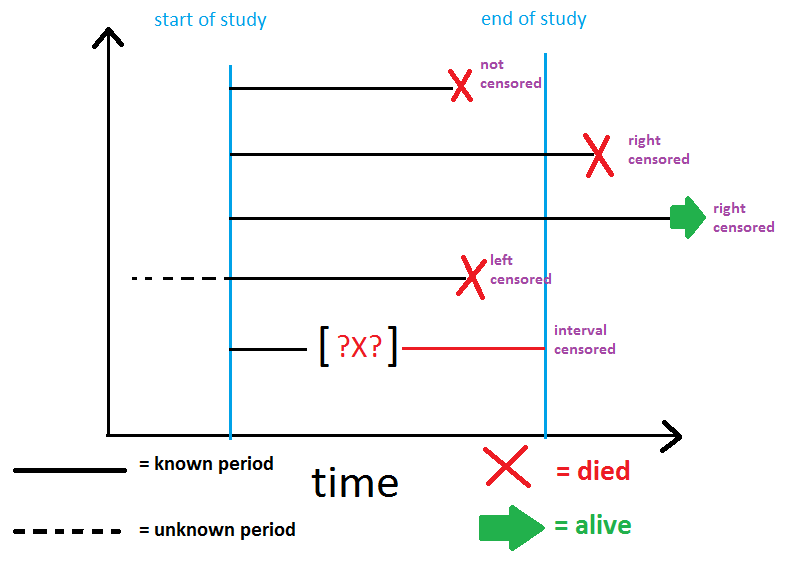
\includegraphics[width=0.75\textwidth]{images/censor.png}
\end{frame}

\begin{frame}{Functions}
\begin{block}{Survival Function}
    \begin{equation*}
        S(t) = P(T \geq t) = \exp[-H(t)]
    \end{equation*}
\end{block}

\begin{block}{Hazard Function}
    \begin{equation*}
        h(t) = \frac{f(t)}{S(t)} = -\frac{d}{dt}[\ln S(t)] \hspace{1cm} H(t) = \int^t_0 h(u) du
    \end{equation*}
\end{block}
\cite{ReddyLi}
\end{frame}

\begin{frame}{Kaplan-Meier Curve}
\begin{columns}
    \begin{column}{0.49\textwidth}
    \begin{itemize}
        \item Non-Parametric Estimate
        \begin{equation*}
        \hat{S}(t) = \prod_{j:T_j<t} \left(1-\frac{d_j}{r_j}\right) 
        \end{equation*}
        \item $r_j$: number of individuals at risk prior to time $T_j$
        \item $d_j$: number of events at $T_j$
        \item Confidence Interval: Log-Log
    \end{itemize}
    
    \end{column}
    \begin{column}{0.49\textwidth}
        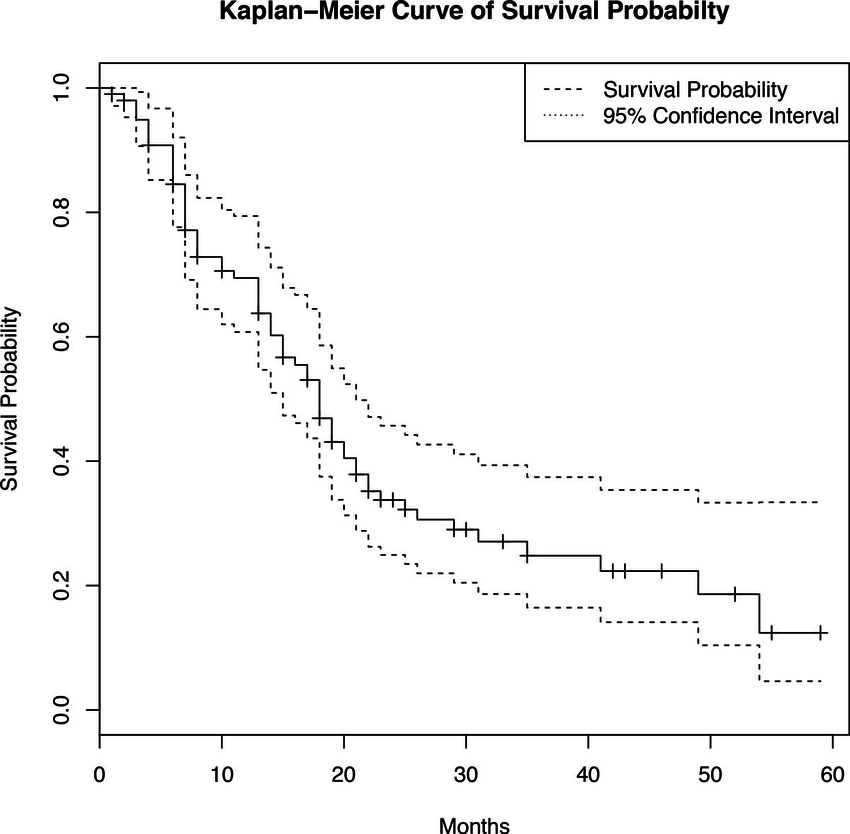
\includegraphics[width = \textwidth]{images/kmc.png}
    \end{column}
\end{columns}
\end{frame}

\begin{frame}{Logrank Test}
\begin{equation*}
    H_0: h_0(t) = h_1(t) \hspace{1cm} H_1: h_0(t) \neq h_1(t)
\end{equation*}

\begin{equation*}
    \chi^2_{logrank} = \frac{\left[\sum^k_{j=1}\left(d_{0j}-\frac{r_{0j}d_j}{r_j}\right)\right]^2}{\sum^k_{j=1}\frac{r_{1j}r_{0j}d_j(r_j-d_j)}{r^2_j(r_j-1)}}
\end{equation*}

\cite{FlemingHarrington}
\end{frame}

\begin{frame}{Cox-Proportional Hazards Model}
    \begin{block}{Cox-Proportional Hazards Model}
        \begin{equation*}
            h(t|X_i) = h_0(t) \exp[X_i\beta]
        \end{equation*}
        \begin{equation*}
        S(t|X_i) = \exp[-H_0(t) \exp(X_i\beta)]
    \end{equation*}
    \end{block}
\end{frame}


\section{Machine Learning Methods}
\begin{frame}{Software}
Python
\begin{itemize}
\item pandas
\item numpy
\item scikit-learn
\item scikit-survival
\end{itemize}

\end{frame}

\begin{frame}{Survival Trees}
\begin{columns}
    \begin{column}{.49\textwidth}
    \begin{itemize}
    \item Splitting Criterion
    \item Prediction
    \item Cross Validation
    \item Pruning
    \end{itemize}
    \cite{SafavianLandgrebe}
    \end{column}
    \begin{column}{.49\textwidth}
    \centering
    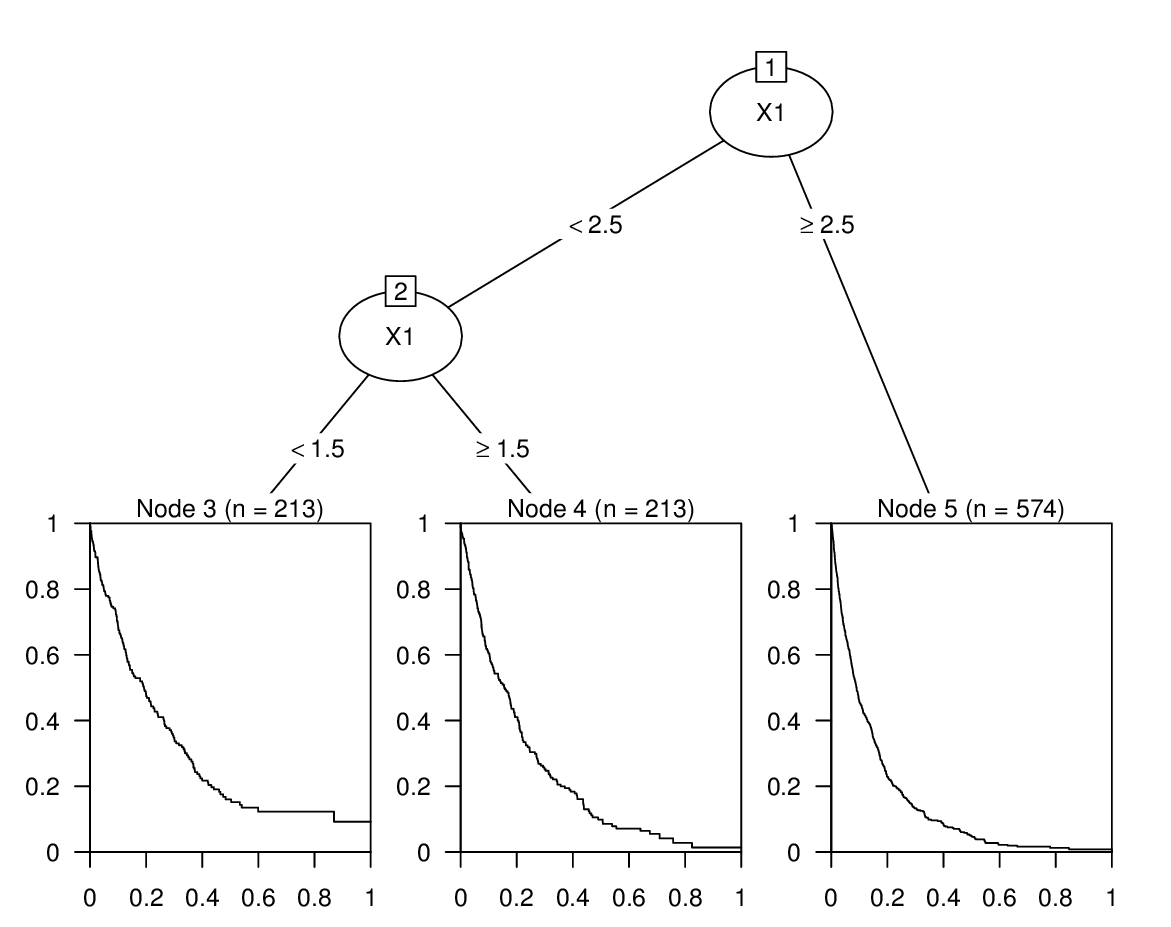
\includegraphics[width = \textwidth]{images/st.png}
    \end{column}
\end{columns}

\end{frame}

\begin{frame}{Random Survival Forest}
\begin{columns}
    \begin{column}{.49\textwidth}
    \begin{itemize}
    \item Ensemble of Survival Trees
    \item Bagging
    \item Subspace Sampling
    \item Feature Importance
    \item Prediction
    \end{itemize}
    \cite{IshwaranEtAl}
    \end{column}
    \begin{column}{.49\textwidth}
    \centering
    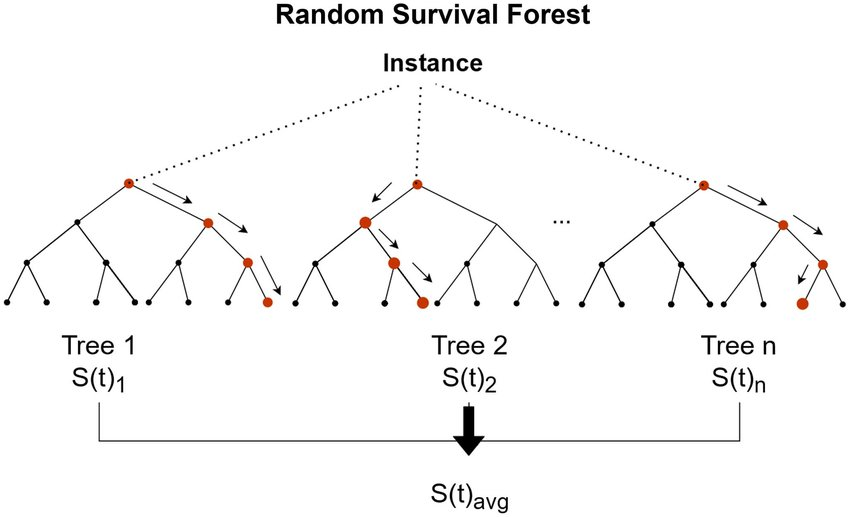
\includegraphics[width = \textwidth]{images/rsf.png}
    \end{column}
\end{columns}

\end{frame}

\begin{frame}{Support Vector Machine (SVM)}
\begin{columns}
    \begin{column}{0.49 \textwidth}
    \begin{itemize}
        \item Hyperplane
        \item Kernels
        \item Regularization
    \end{itemize}
    \cite{WangEtAl}
    \end{column}
    \begin{column}{0.49 \textwidth}
        \centering
        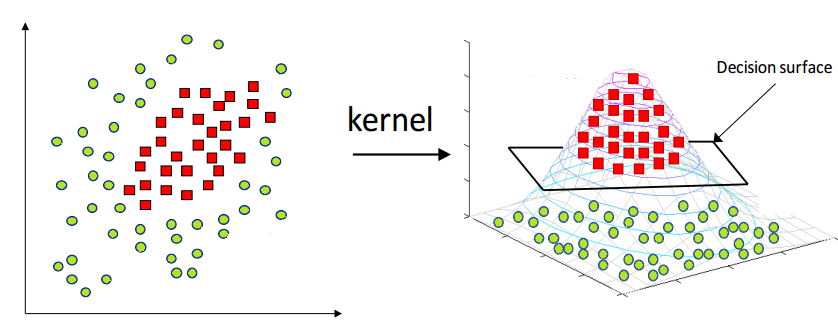
\includegraphics[width = \textwidth]{images/svm.png}
    \end{column}
\end{columns}
\end{frame}

\begin{frame}{Neural Networks}
\begin{columns}
    \begin{column}{0.49 \textwidth}
    \begin{itemize}
        \item Censored Data
        \item Survival Loss Functions
        \item CNNs, RNNs
    \end{itemize}
        \cite{WangEtAl}
    \end{column}
    \begin{column}{0.49 \textwidth}
        \centering
        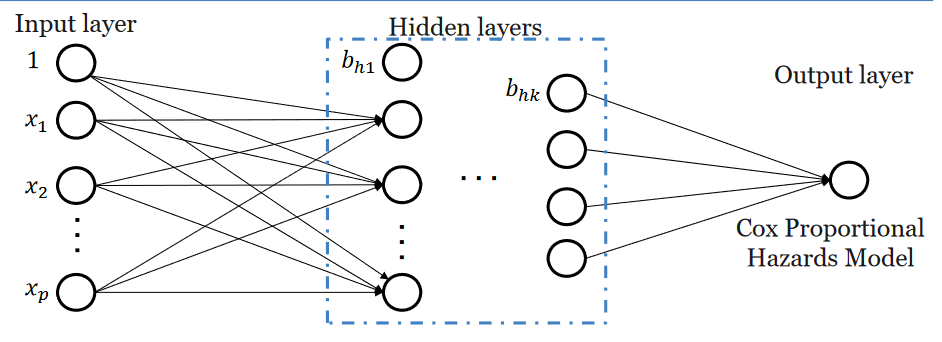
\includegraphics[width=\textwidth]{images/nn.png}
    \end{column}
\end{columns}
\end{frame}

\begin{frame}{Evaluation Metrics I}

\begin{block}{Concordance Index}
\begin{align*}
    \hat{c} &= \frac{1}{num} \sum_{i: \delta_i = 1} \sum_{j:y_i<y_j} I[\hat{S}(y_i|X_i) < \hat{S}(y_j|X_j)] \\
    &= \frac{1}{num} \sum_{i: \delta_i = 1}\sum_{j:y_i<y_j}  I[X_i\hat{\beta} > X_j \hat{\beta}]
\end{align*}
\end{block}

\cite{UnoEtAl}

\end{frame}

\begin{frame}{Evaluation Metrics II}
\begin{block}{Integrated Brier Score}
\begin{align*}
    IBS &= \int^{t_k}_{t_1}BS(t)dt\\
    BS(t) &= \frac{1}{n}\sum^n_{i=1}\left[\hat{S}(t|X_i)-I[T_i > t]\right]^2
\end{align*}
\end{block}

\cite{GrafEtAl}
\end{frame}

\begin{frame}{Evaluation Metrics III}
\begin{block}{Cumulative/Dynamic AUC}
\begin{equation*}
    AUC(t) = \frac{\sum^n_{i=1} \sum^{n}_{j=1} I[T_i>t]I[T_j\leq t] I[\hat{S}(t|X_i) \geq \hat{S}(t|X_j)]}{\sum^n_{i=1} \sum^n_{j=1} I[T_i>t]I[T_j \leq t]}
\end{equation*}
\end{block}

\cite{UnoEtAl}
\end{frame}

\section{Real Dataset}

\begin{frame}{Breast Cancer Gene Expression Profiles (METABRIC)
}
\begin{columns}
    \begin{column}{0.49\textwidth}
        \centering
        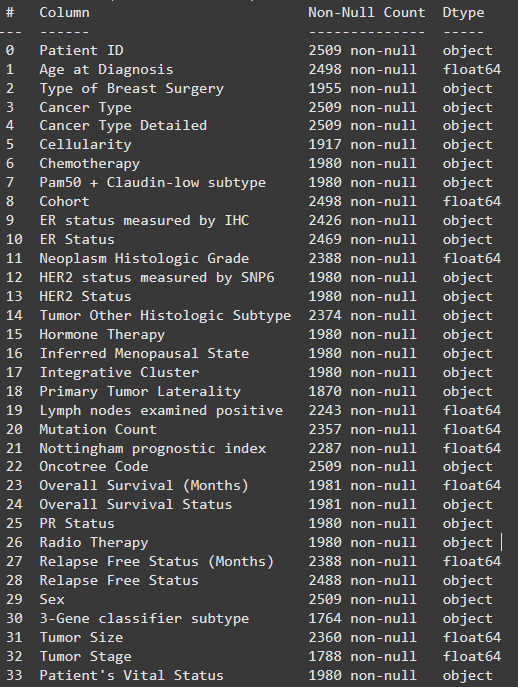
\includegraphics[width=.95\textwidth]{images/eda1.png}
    \end{column}
    \begin{column}{0.49\textwidth}
        \begin{itemize}
            \item 2,509 Breast Cancer Patients
            \item 30 Features
            \item Overall Survival Status
            \item Overall Survival (Months)
            \item Relapse Free Status
            \item Relapse Free Status (Months)
        \end{itemize}
    \end{column}
\end{columns}
\end{frame}

\begin{frame}{EDA I}
    \centering
    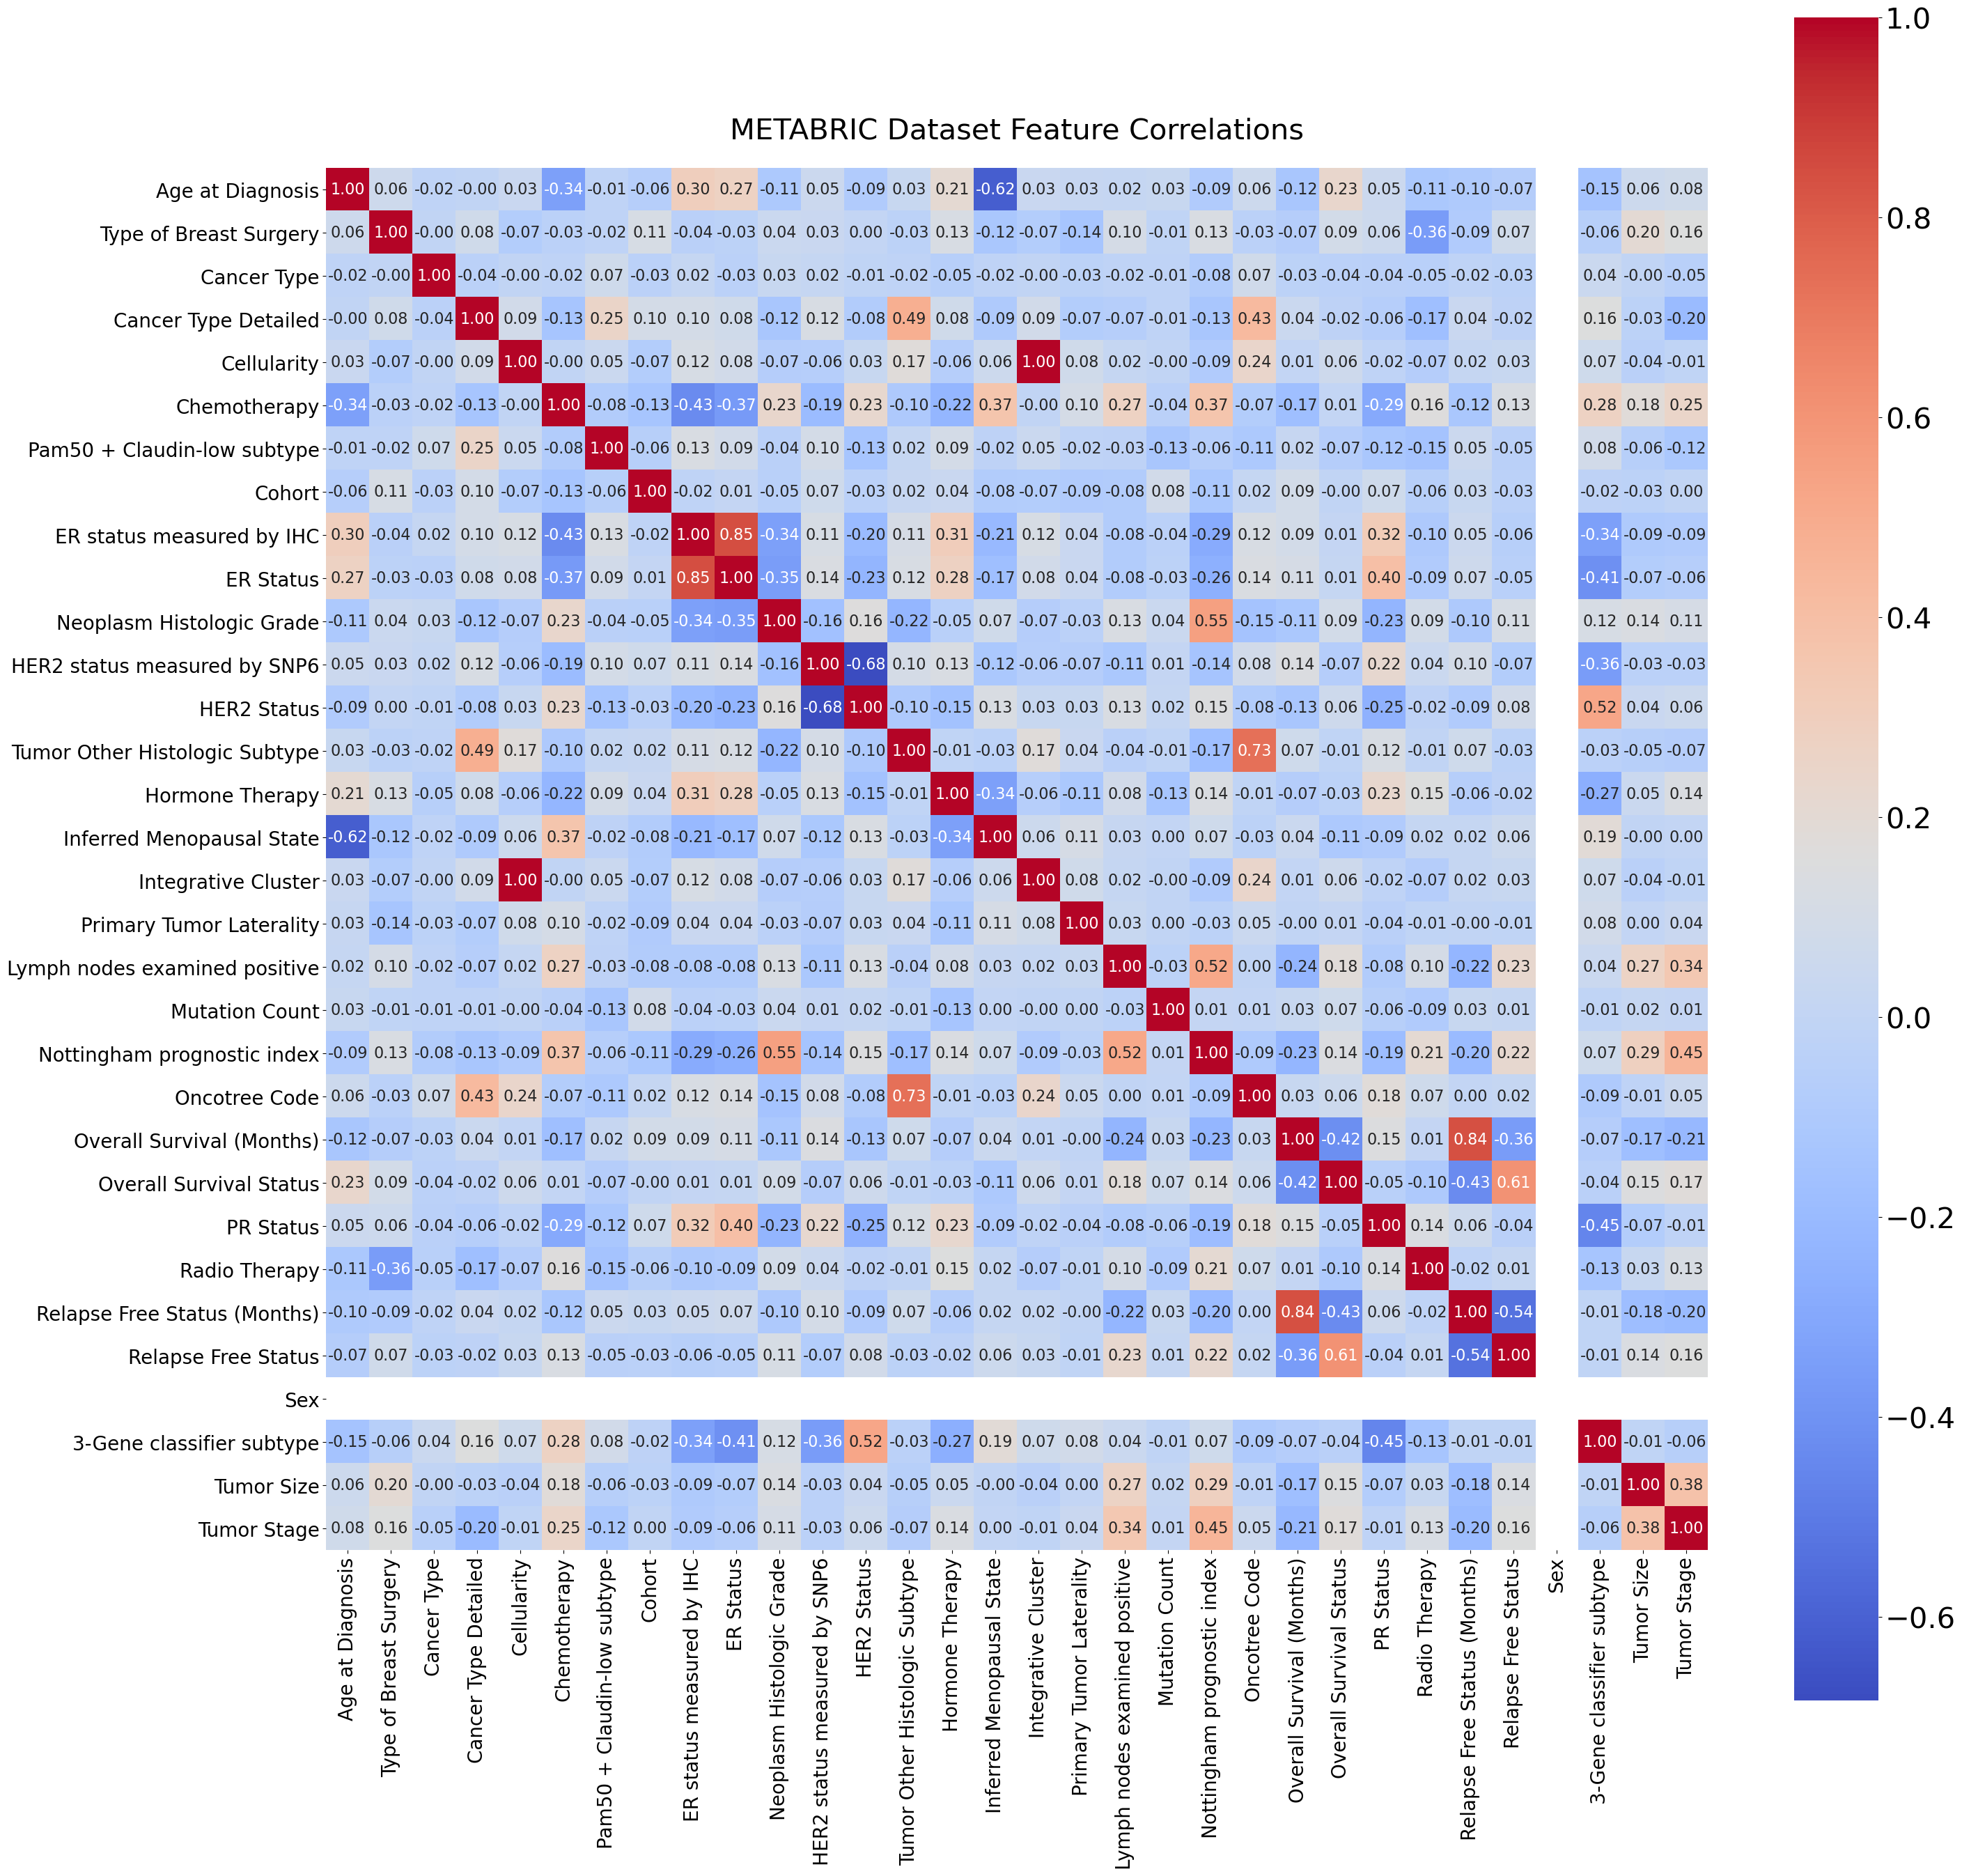
\includegraphics[width = 0.8\textwidth]{images/corr.png}
\end{frame}

\begin{frame}{EDA II}
\begin{columns}
    \begin{column}{0.49 \textwidth}
        \centering
        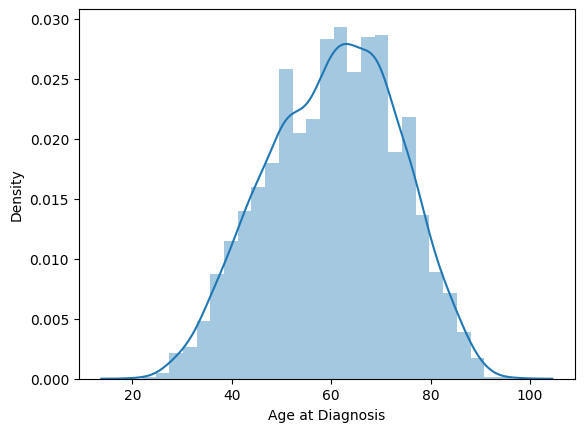
\includegraphics[width = \textwidth]{images/age.png}
    \end{column}
    \begin{column}{0.49 \textwidth}
        \centering
        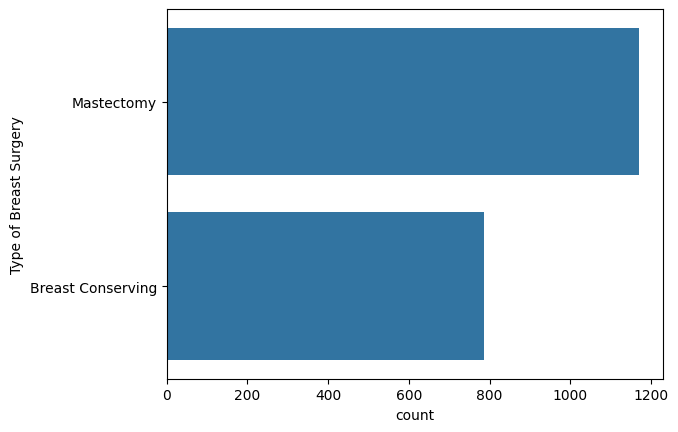
\includegraphics[width = \textwidth]{images/breast_surgery.png}
    \end{column}
\end{columns}
\end{frame}

\begin{frame}{EDA III}
\begin{columns}
    \begin{column}{0.49 \textwidth}
        \centering
        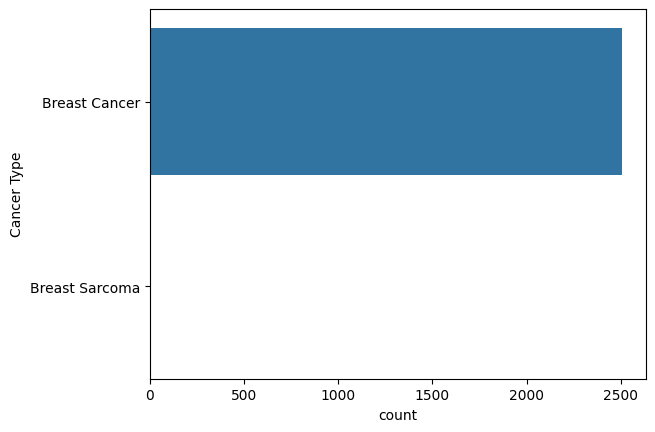
\includegraphics[width = \textwidth]{images/c_type.png}
    \end{column}
    \begin{column}{0.49 \textwidth}
        \centering
        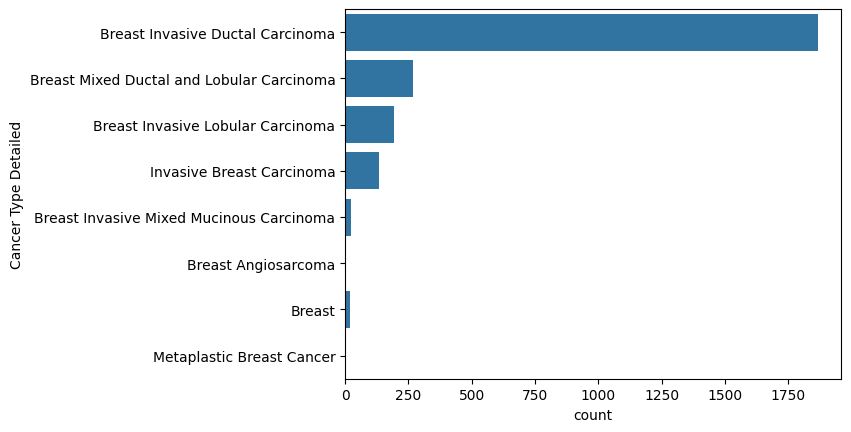
\includegraphics[width = \textwidth]{images/cancer types.png}
    \end{column}
\end{columns}
\end{frame}

\begin{frame}{EDA IV}
    \centering
    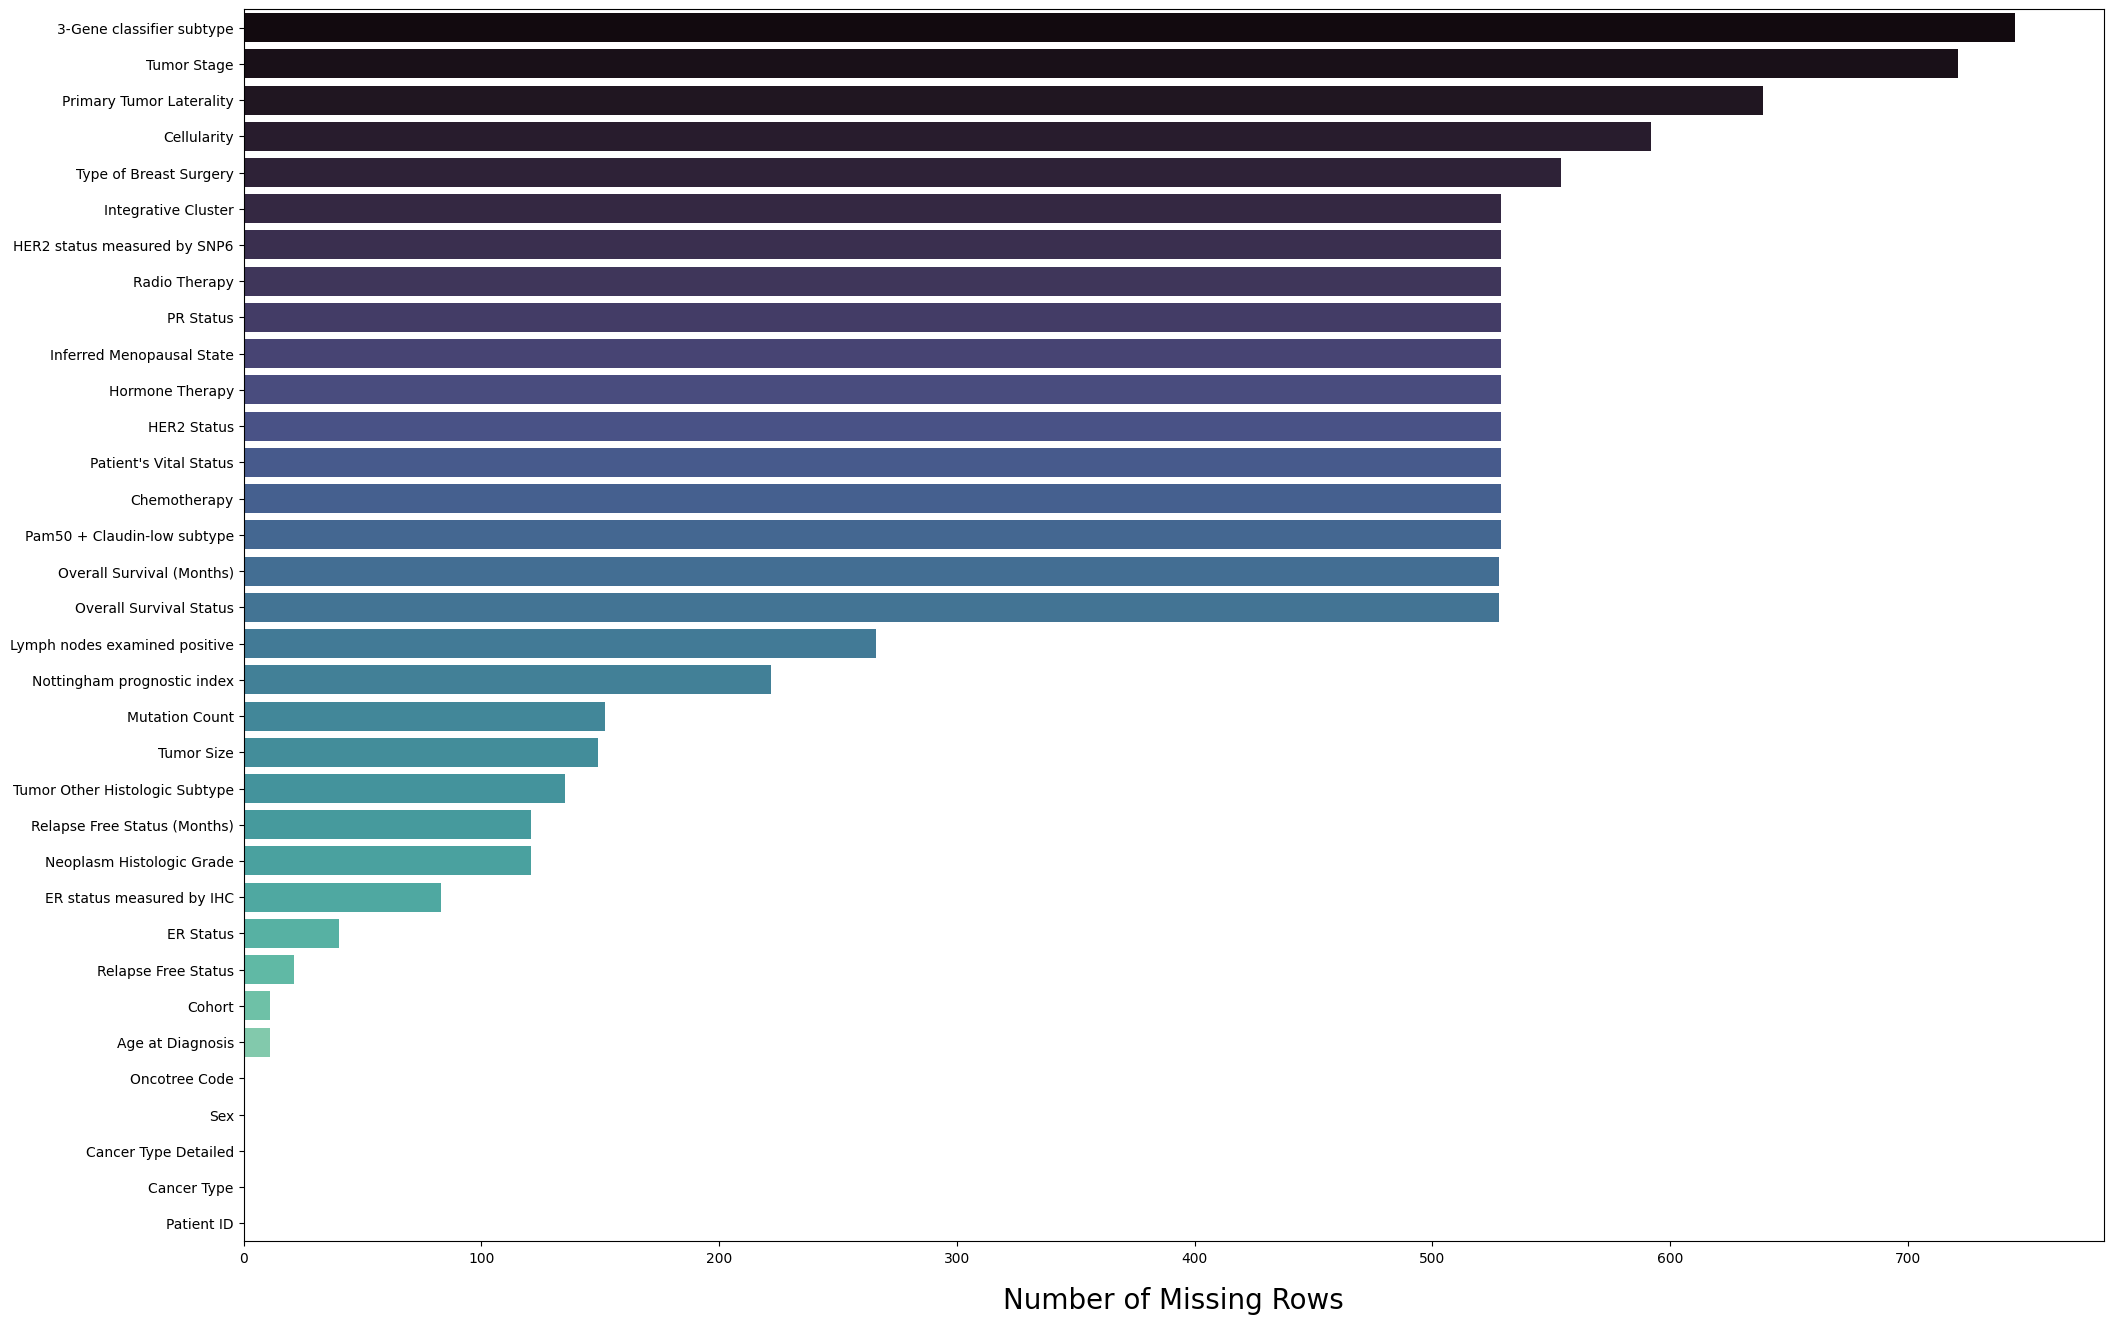
\includegraphics[width = \textwidth]{images/missing.png}
\end{frame}

\begin{frame}{EDA V}
\begin{columns}
    \begin{column}{0.49 \textwidth}
        \centering
        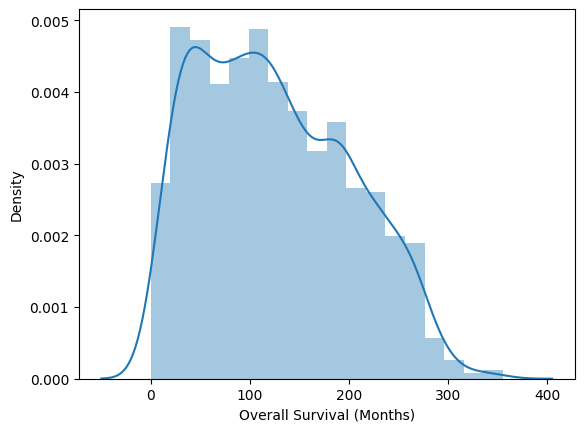
\includegraphics[width = \textwidth]{images/surv_m.png}
    \end{column}
    \begin{column}{0.49 \textwidth}
        \centering
        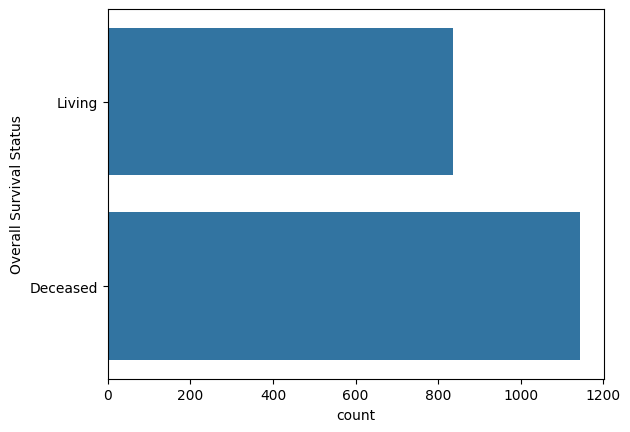
\includegraphics[width = \textwidth]{images/surv_s.png}
    \end{column}
\end{columns}
\end{frame}

\begin{frame}{EDA VI}
\begin{columns}
    \begin{column}{0.49 \textwidth}
        \centering
        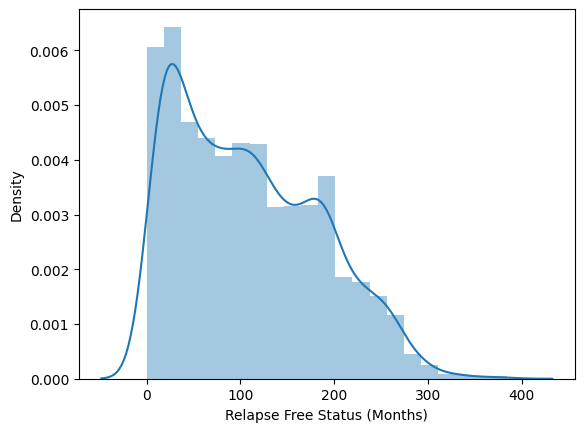
\includegraphics[width = \textwidth]{images/relapse_m.png}
    \end{column}
    \begin{column}{0.49 \textwidth}
        \centering
        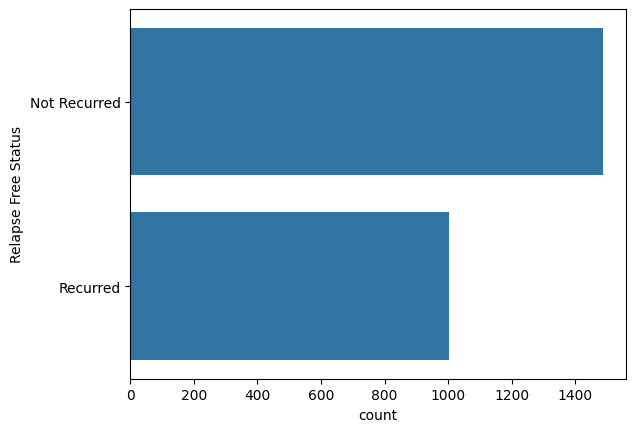
\includegraphics[width = \textwidth]{images/relapse_s.png}
    \end{column}
\end{columns}
\end{frame}

\begin{frame}{Pre-processing}
    \begin{columns}
        \begin{column}{0.49 \textwidth}
            Feature Removal:
            \begin{itemize}
                \item Patient ID
                \item Cancer Type
                \item Sex
                \item Integrative Cluster
                \item Patient's Vital Status
            \end{itemize}
        \end{column}
        \begin{column}{0.49 \textwidth}
            Complete Dataset
            \begin{itemize}
                \item 1092 Instances
                \item 8 Numerical
                \item 16 Nominal
                \item 1 Ordinal
                \item 4 Labels
                \item 45 Features
            \end{itemize}
        \end{column}
    \end{columns}
\end{frame}

\begin{frame}{Kaplan Meier Curve}
    \centering
    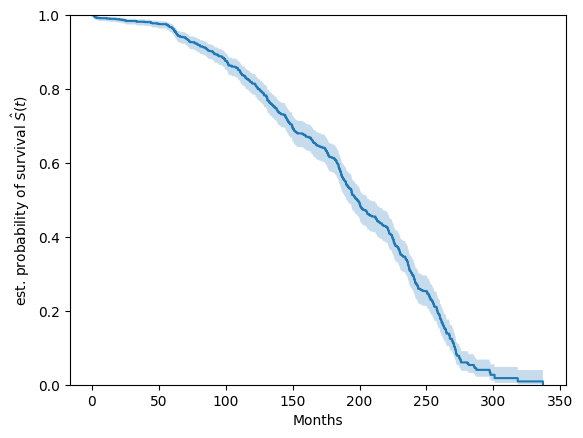
\includegraphics[width = 0.75\textwidth]{images/kmc_r.png}
\end{frame}

\begin{frame}{Cox-Proportional Hazards Model I}
    \begin{columns}
        \begin{column}{0.49 \textwidth}
            \centering
            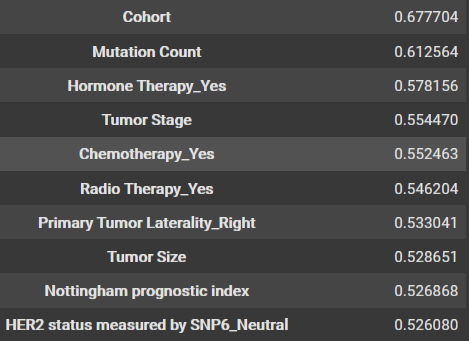
\includegraphics[width = \textwidth]{images/single.png}
        \end{column}
        \begin{column}{0.49 \textwidth}
            \begin{itemize}
                \item Cohort: -0.497392
                \item Mutation Count: -0.141548
                \item Hormone Therapy\_Yes: 0.378709
                \item Tumor Stage: 0.076158
                \item Chemotherapy\_Yes: 0.493760
		\item Radio Therapy\_Yes: 0.293066
		\item Primary Tumor Laterality\_Right: 0.121881
            \end{itemize}
        \end{column}
    \end{columns}
\end{frame}

\begin{frame}{Cox-Proportional Hazards Model II}
    \begin{columns}
        \begin{column}{0.49 \textwidth}
            \centering
            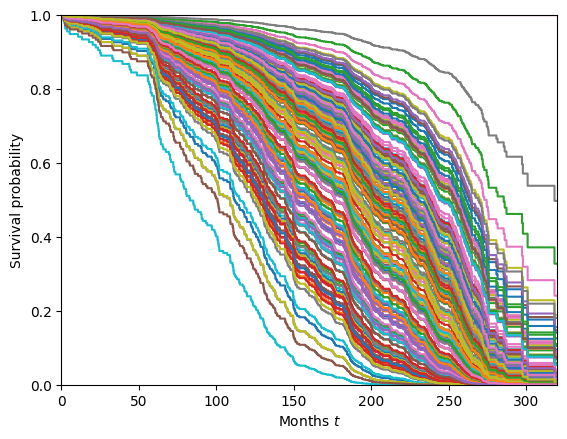
\includegraphics[width = \textwidth]{images/cox_sf.png}
        \end{column}
        \begin{column}{0.49 \textwidth}
            \centering
            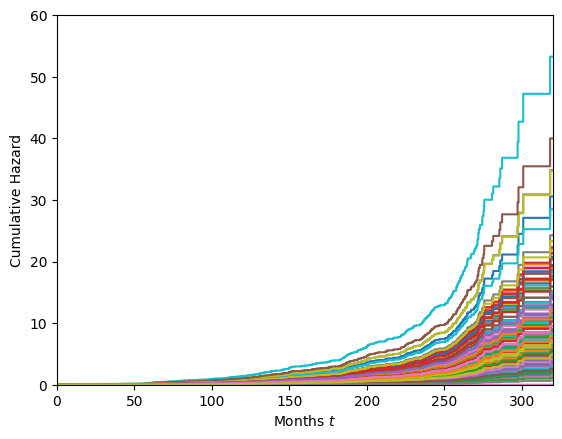
\includegraphics[width = \textwidth]{images/cox_chf.png}
        \end{column}
    \end{columns}
\end{frame}

\begin{frame}{Cox-Proportional Hazards Model III}
    \begin{columns}
        \begin{column}{0.49 \textwidth}
            \begin{itemize}
                \item C-Index: 0.7159
                \item Integrated Brier Score: 0.12082
                \item Cumulative AUC Mean: 0.76155
            \end{itemize}
        \end{column}
        \begin{column}{0.49 \textwidth}
            \centering
            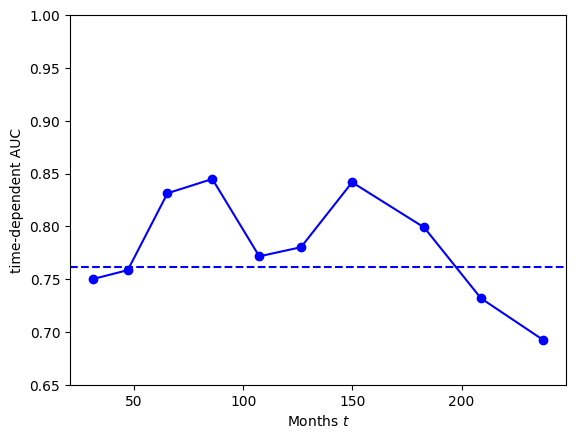
\includegraphics[width = \textwidth]{images/cox_auc.png}
        \end{column}
    \end{columns}
\end{frame}


\begin{frame}{Log Rank Test I}
    \begin{columns}
        \begin{column}{0.49 \textwidth}
        Hormone Therapy
        \begin{itemize}
            \item $\chi^2$: 19.87413
            \item p-value: 8.27119e-06
        \end{itemize}
        \end{column}
        \begin{column}{0.49 \textwidth}
            \centering
            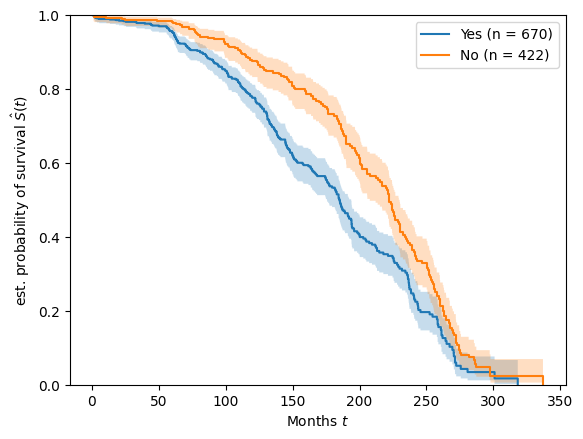
\includegraphics[width = \textwidth]{images/logrank1}
        \end{column}
    \end{columns}
\end{frame}

\begin{frame}{Log Rank Test II}
    \begin{columns}
        \begin{column}{0.49 \textwidth}
        Chemotherapy
        \begin{itemize}
            \item $\chi^2$: 36.52974
            \item p-value: 1.50354e-09
        \end{itemize}
        \end{column}
        \begin{column}{0.49 \textwidth}
            \centering
            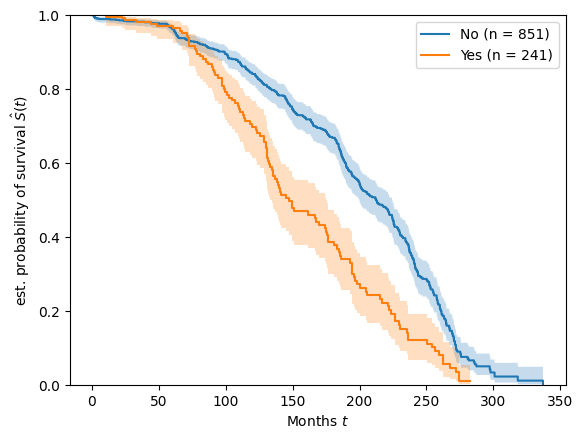
\includegraphics[width = \textwidth]{images/logrank2}
        \end{column}
    \end{columns}
\end{frame}

\begin{frame}{Log Rank Test III}
    \begin{columns}
        \begin{column}{0.49 \textwidth}
        Radio Therapy
        \begin{itemize}
            \item $\chi^2$: 18.00271
            \item p-value: 2.20590e-05
        \end{itemize}
        \end{column}
        \begin{column}{0.49 \textwidth}
            \centering
            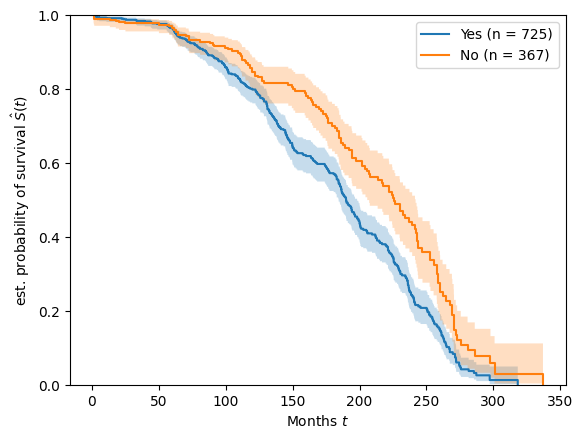
\includegraphics[width = \textwidth]{images/logrank3}
        \end{column}
    \end{columns}
\end{frame}

\begin{frame}{Log Rank Test IV}
    \begin{columns}
        \begin{column}{0.49 \textwidth}
        Primary Tumor Laterality
        \begin{itemize}
            \item $\chi^2$: 10.73803
            \item p-value: 0.01323
        \end{itemize}
        \end{column}
        \begin{column}{0.49 \textwidth}
            \centering
            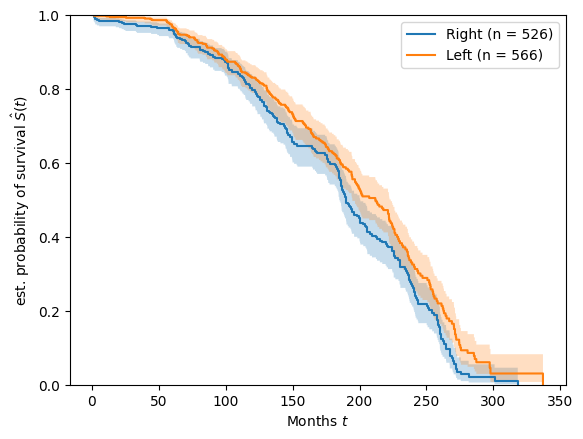
\includegraphics[width = \textwidth]{images/logrank4}
        \end{column}
    \end{columns}
\end{frame}

\begin{frame}{Survival Tree I}
    \begin{columns}
        \begin{column}{0.49 \textwidth}
            \begin{itemize}
                \item Cross Validaion: 5 Fold
                \item Max Depth: 8
                \item Min Samples Leaf: 40
                \item 17 Leafs
            \end{itemize}
        \end{column}
        \begin{column}{0.49 \textwidth}
            \centering
            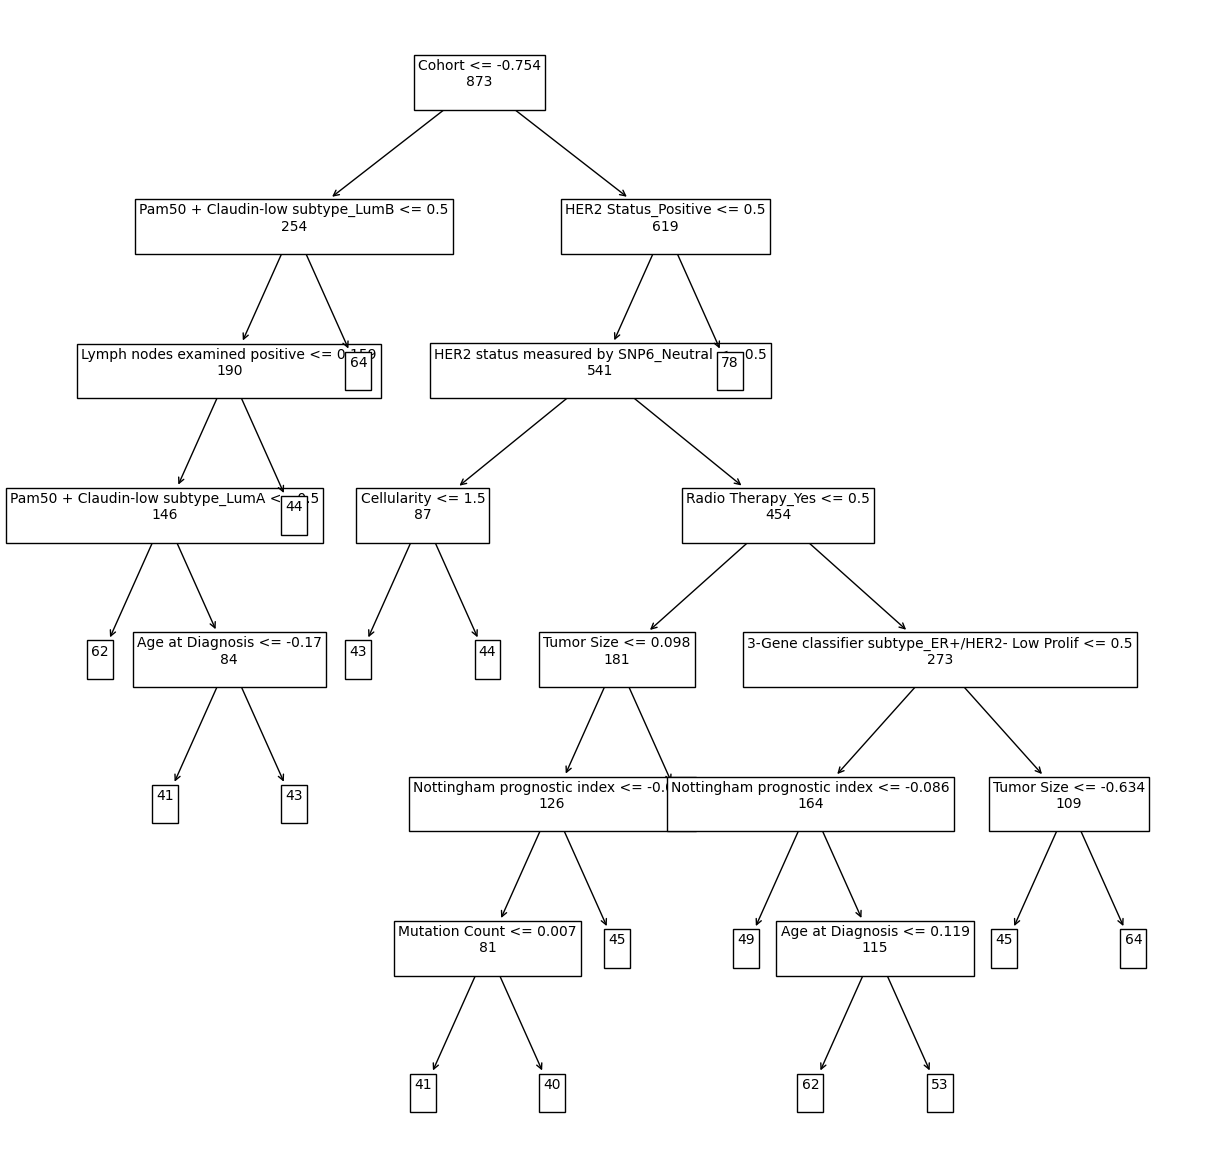
\includegraphics[width = \textwidth]{images/st_tree.png}
        \end{column}
    \end{columns}
\end{frame}

\begin{frame}{Survival Tree II}
    \begin{columns}
        \begin{column}{0.49 \textwidth}
            \centering
            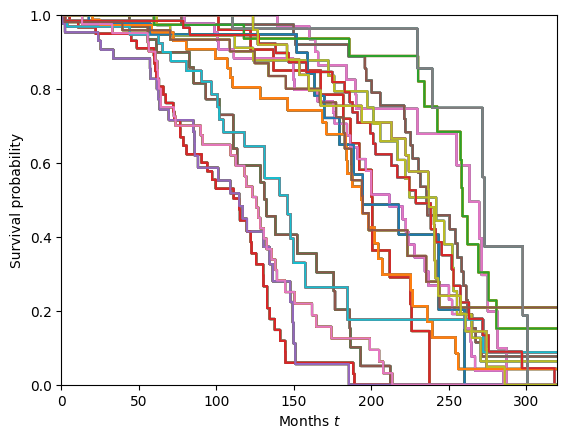
\includegraphics[width = \textwidth]{images/st_sf.png}
        \end{column}
        \begin{column}{0.49 \textwidth}
            \centering
            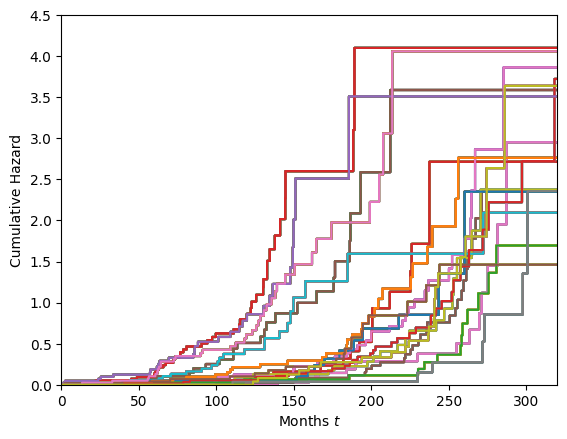
\includegraphics[width = \textwidth]{images/st_chf.png}
        \end{column}
    \end{columns}
\end{frame}

\begin{frame}{Survival Tree III}
    \begin{columns}
        \begin{column}{0.49 \textwidth}
            \begin{itemize}
                \item C-Index: 0.71565
                \item Integrated Brier Score: 0.11133
                \item Cumulative AUC Mean: 0.76799
            \end{itemize}
        \end{column}
        \begin{column}{0.49 \textwidth}
            \centering
            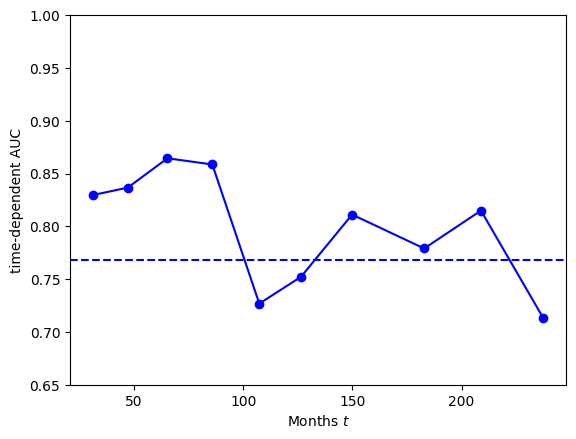
\includegraphics[width = \textwidth]{images/st_auc.png}
        \end{column}
    \end{columns}
\end{frame}

\begin{frame}{Random Survival Forest I}
    \begin{columns}
        \begin{column}{0.49 \textwidth}
		\begin{itemize}
		\item Cross-Validation: 5 Fold
		\item Max Depth: 6
		\item Min Samples Leaf: 10
		\end{itemize}
        \end{column}
        \begin{column}{0.49 \textwidth}
            \centering
            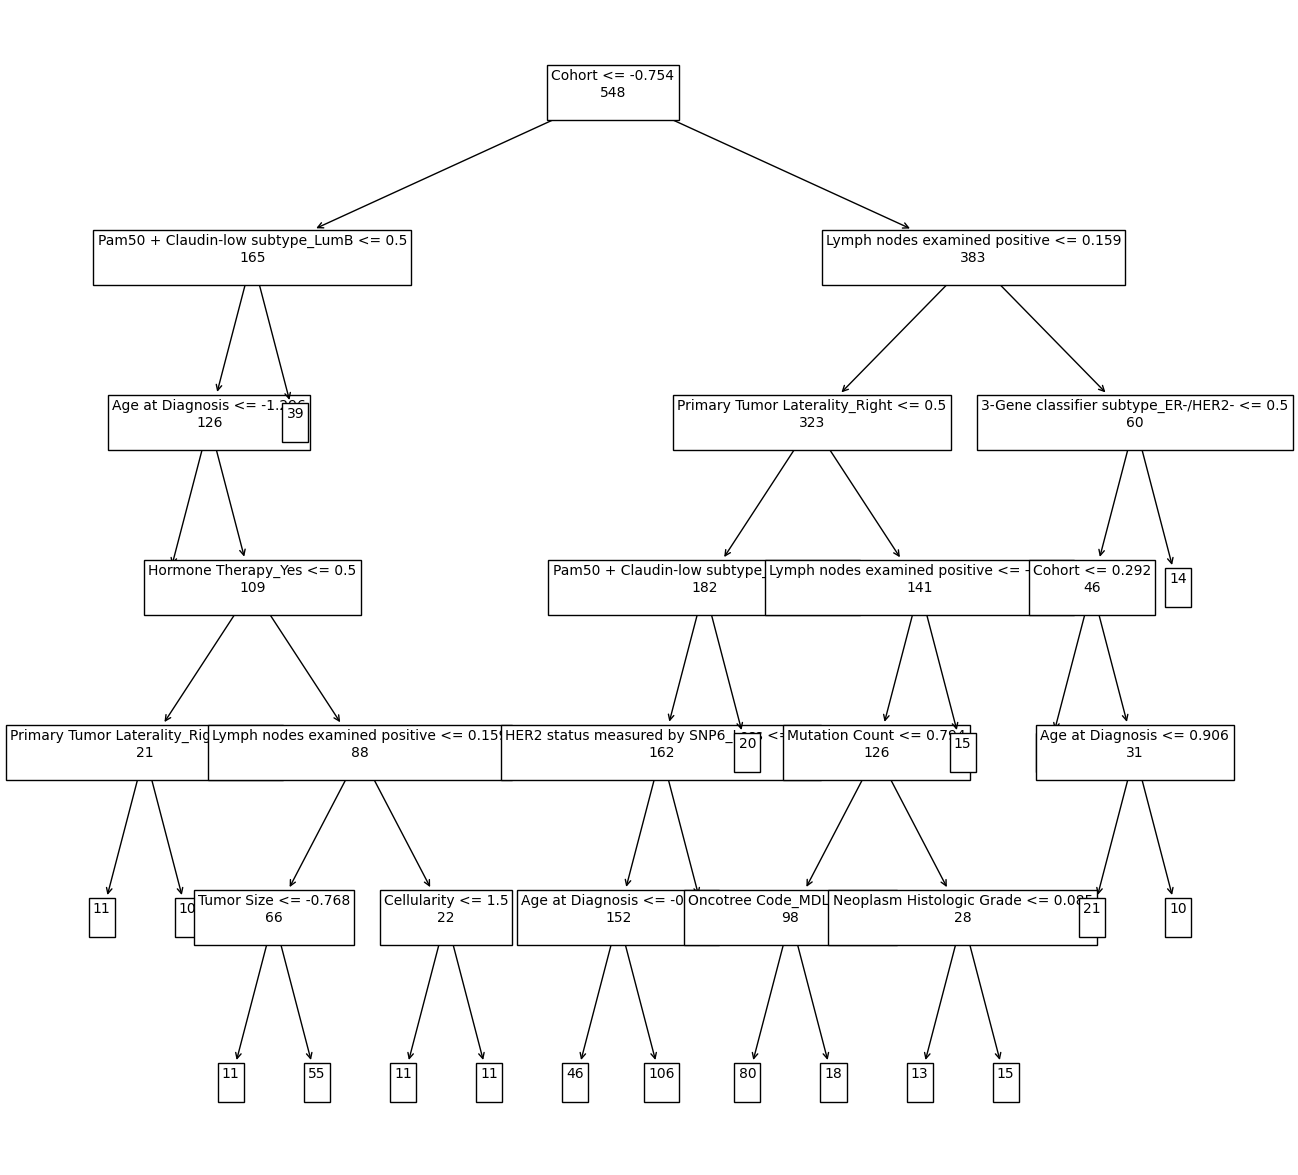
\includegraphics[width = \textwidth]{images/rsf_tree.png}
        \end{column}
    \end{columns}
\end{frame}

\begin{frame}{Random Survival Forest II}
    \begin{columns}
        \begin{column}{0.49 \textwidth}
            \centering
            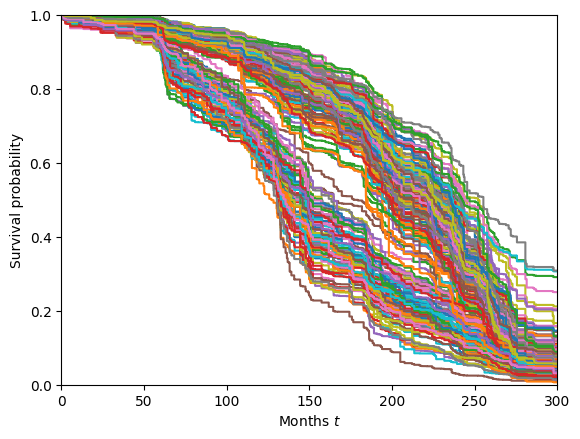
\includegraphics[width = \textwidth]{images/rsf_sf.png}
        \end{column}
        \begin{column}{0.49 \textwidth}
            \centering
            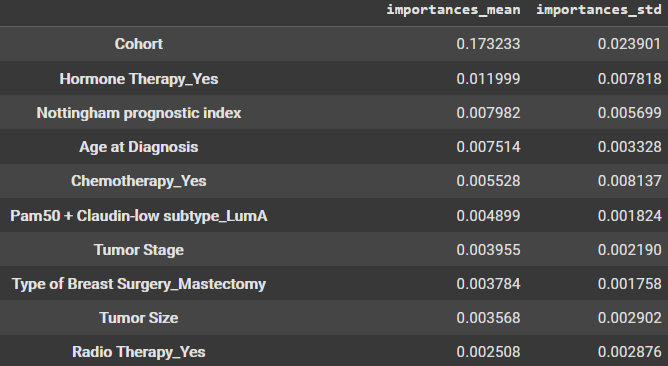
\includegraphics[width = \textwidth]{images/rsf_fi.png}
        \end{column}
    \end{columns}
\end{frame}

\begin{frame}{Random Survival Forest III}
    \begin{columns}
        \begin{column}{0.49 \textwidth}
            \begin{itemize}
                \item C-Index: 0.75570
                \item Integrated Brier Score: 0.10784
                \item Cumulative AUC Mean: 0.81813
            \end{itemize}
        \end{column}
        \begin{column}{0.49 \textwidth}
            \centering
            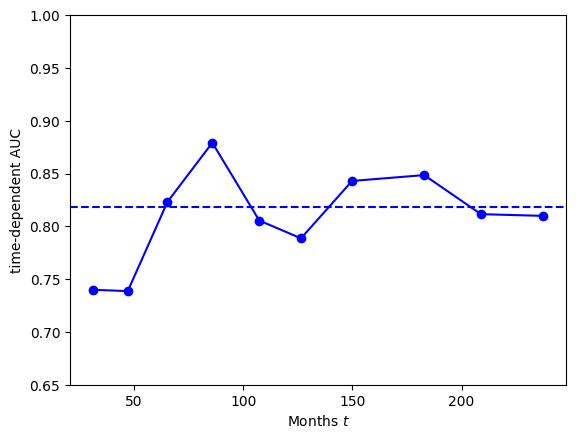
\includegraphics[width = \textwidth]{images/rsf_auc.png}
        \end{column}
    \end{columns}
\end{frame}

\begin{frame}{SVM}
    \begin{columns}
        \begin{column}{0.49 \textwidth}
            \begin{itemize}
                \item alpha: 0.0625
                \item C-Index: 0.72064
                \item Cumulative AUC Mean: 0.76021
            \end{itemize}
        \end{column}
        \begin{column}{0.49 \textwidth}
            \centering
            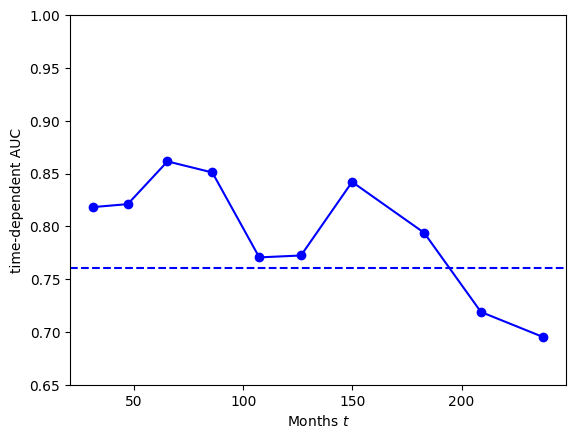
\includegraphics[width = \textwidth]{images/svm_r.png}
        \end{column}
    \end{columns}
\end{frame}


\section{Conclusion}
\begin{frame}{Conclusion}
\begin{itemize}
\item Survival Analysis
\item Machine Learning
\item Real Data Analysis
\end{itemize}
\end{frame}

\begin{frame}{Future Work}
\begin{itemize}
    \item Imputation
    \item Relapse Free Status
	\item Other ML Methods \cite{WangEtAl}:
\begin{itemize}
    \item Neural Networks
    \item Gradient Boosting
	\item Bagging Survival Trees
\end{itemize}
\end{itemize}
\end{frame}


\begin{frame}[allowframebreaks]{References}
    \bibliographystyle{apalike}
    \bibliography{./ref.bib}
\end{frame}


\end{document}